\chapter{Introducción}
	
	El caos se refiere a un tipo de comportamiento dinámico complejo que posee algunas características muy especiales, tales como extrema sensibilidad a pequeñas variaciones de la condición inicial, trayectorias encerradas en el espacio de fase pero con un exponente de Lyapunov positivo, un espectro de potencia continuo entre muchas otras. En pocas palabras, el caos es simplemente un comportamiento impredecible de un sistema determinista. Es de interés resaltar que los sistemas caóticos ya eran conocidos desde hace mucho tiempo atrás y que no fue hasta hace poco que se logró demostrar que el caos puede ser controlado y debido a esto impactar en muchas áreas, tanto en áreas cercanas a la electrónica como técnicas de modulación, sistemas de comunicación, técnicas de encriptación de datos, como también en áreas  relacionadas a los sistemas biológicos, reacciones químicas, toma de decisiones críticas en política, economía, eventos militares, etc  \cite{Munoz-Pacheco2010}. El caos es un fenómeno que ocurre en muchos sistemas no lineales, donde la naturaleza determinista de la estructura se conjuga con la irregularidad del comportamiento, esto significa que, a pesar del hecho de que el sistema se describe mediante un conjunto de ecuaciones diferenciales ordinarias, donde todos los términos son perfectamente conocidos, su comportamiento es irregular y muy sensible a las condiciones iniciales. La primera evidencia de imprevisibilidad en los sistemas deterministas se encuentra en el trabajo del matemático y científico Henri Poincaré sobre el movimiento celestial, mientras que la primera formulación del caos en un modelo matemático expresado por un conjunto de ecuaciones diferenciales ordinarias que exhiben el caos se debe al matemático y meteorólogo Edward Lorenz que estaba estudiando un modelo de movimiento del aire en la atmósfera y descubrió cómo pequeñas variaciones en los valores iniciales de las variables de su modelo dieron como resultado predicciones meteorológicas divergentes \cite{Buscarino2014}. Para el momento de esos estudios faltaba una prueba experimental definitiva del caos y la tecnología y poder de cómputo no eran suficientes para pensar aún en soluciones y aún más distantes las aplicaciones. Debido al constante avance de la electrónica, hoy en día somos capaces de sintetizar mediante dispositivos electrónicos sistemas caóticos, utilizando técnicas de modelado e implementación es posible crear representaciones de estos, no obstante, todas estas se basan en aproximaciones que aún no han sido exploradas en su totalidad. 
	Por otro lado el cálculo fraccionario es un tema que tiene más de 300 años de antigüedad y que se remonta a cartas enviadas a Leibniz por parte de Bernoulli y de L'Hôspital preguntando acerca de la derivada a la $1/2$ e indagando sobre su significado. Con el paso de los años la teoría de cálculo fraccionario se fue desarrollando pasando por las manos de nombres conocidos como: Euler, Lagrange, Laplace, Fourier hasta llegar a Liouville, Riemann, Grünwald, Letnikov, Caputo entre muchos otros \cite{Petras2011}. Pero aún con todo ese desarrollo no fue hasta hace poco que la comunidad científica comenzó a interesarse por esta rama del cálculo y la razón principal de este cambio es que los cálculos necesarios para cualquier posible implemetación eran demasiado complejos y lentos, un panorama totalmente diferente se vive en la actualidad, el rápido avance de la tecnología ha logrado realizar avances notables en esta área. El rango de aplicaciones para el cálculo fraccionario es inmenso, por mencionar algunas de las más recientes, la modelación de derivadas fraccionarias para obtener una mejor representación comportamental de un sistema industrial metalúrgico \cite{Petras2019}, la incorporación de dinámica de orden fraccional para mejorar la robustez de un control PI/PID para motores DC \cite{Tepljakov2016,Khubalkar2018}, la modelación de señales biológicas como ECG, EMG y EEG debido a su respuesta de magnitud de 20$\alpha$dB, modelos fisiológicos basados en ecuaciones diferenciales lineales que describen fenómenos complejos en el cuerpo humano como la oxigenación de la sangre entre otros \cite{Ortigueira2011}.
	El cálculo fraccionario y los sistemas caóticos se complementan al añadir un nivel de profundidad en la creación de osciladores caóticos modelados como un conjunto de ecuaciones diferenciales no lineales fraccionarias las cuales son materia prima para la creación de nuevas aplicaciones y áreas de desarrollo. 
	
	\section{Justificación}
	
	Los osciladores caóticos son una área de oportunidad emergente cuyas aplicaciones han aumentado en los ultimamos años, a principios del siglo XX se comenzó a explorar el uso de osciladores caóticos para la detección de señales pequeñas basados en la propiedad  de extrema sensibilidad a pequeños cambios de la condición inicial que estos presentan \cite{Wang1999}, y en la seguridad de sistemas de comunicación ya sea en tiempo continuo o discreto \cite{Tepina2002}.  Casi al mismo tiempo los sistemas de orden fraccionario comenzaron a formar parte del interés de la comunidad científica nuevamente y se abrieron las puertas al control de sistemas de orden fraccionario y como implementarlos \cite{Chen2009,Das2007}. Los intentos de implementaciones físicas de sistemas de orden fraccionario han avanzado mucho recientemente y se pueden categorizar en digitales, los cuales utilizan sistemas discretos basados en microprocesadores o FPGA cuya complejidad radica en poder generar un software robusto que sea lo suficiente fiable \cite{Gunay2017}. Por el otro lado se encuentran las implenetaciones analógicas, las cuales son de gran interés en este trabajo. En la literatura de esta área podemos encontrar implementaciones basadas en la construcción de capacitores electrolíticos especiales que se aproximan al comportamiento fraccionario pero cuya fabricación es compleja \cite{Jesus2008}, métodos electroquímicos que trabajan con compuestos químicos de difícil manipulación y tienen ordenes que no pueden modificarse fácilmente \cite{Biswas2006}, finalmente y en lo que se enfocará este trabajo se encuentran las aproximaciones de funciones racionales en un ancho de banda determinado utilizando los métodos de Newton, Oustaloup, Carlson, Matsuda o expansión de fracciones continuas (CFE) \cite{Charef2006,Krishna2011,Krishna2008}. Una vez que la función de trasferencia es obtenida, esta se sintetiza utilizando diferentes metodologías, como la realización pasiva que hace uso de resistencias, capacitores e inductores, con el inconveniente de poder ajustarse a los valores comerciales, o la realización activa, que utiliza las técnicas de diseño basadas en amplificadores operacionales \cite{Tepljakov2013, Dorcak2012}. Una alternativa a estas metodologías es la sintetización utilizando dispositivos analógicos embebidos programables FPAA (Field Programable Analog Array). Las FPAA han demostrado ser una arquitectura prometedora que facilita mucho el proceso de implemetación de circuitos analógicos debido a que su interfaz se basa en Módulos Analógicos Configurables (CAM), los cuales son bloques que pueden interconectarse fácilmente y representan desde circuitos sencillos como integradores, derivadores, sumadores o inversores hasta circuitos más complejos como filtros completos y multiplicadores \cite{Fragoulis2009}. Sin embargo en el ámbito tanto de integradores fraccionarios como de osciladores caóticos aun existen metodologías nuevas por explorar, en algunos artículos científicos ya se ha mostrado como implementar un integrador de orden fraccionario utilizando la aproximación de Oustaloup y CAMs de filtros bilineales \cite{Caponetto2006}, no obstante la cantidad de recursos para crear un solo integrador es muy grande, lo cual da pie a ser mejorado utilizando aproximaciones diferentes, por ejemplo la expansión de fracciones continuas. De mismo modo implementar osciladores caóticos basados en sistemas de ecuaciones diferenciales de orden entero utilizando una FPAA ya ha sido explorado en años recientes \cite{Caponetto2006,Li2018}, sin embargo los basados en sistemas de ecuaciones diferenciales de orden fraccionario aun se encuentran en una etapa temprana y son ideales para ser estudiados. Las aplicaciones de los osciladores caóticos van en aumento y ser capaces de implemetarlos se ha vuelto una tarea relevante, estos ahora se están utilizando en aplicaciones médicas, como en la detección de señales cardíacas \cite{Jiang2010} y en la creación de radares UWB que tienen futuro prometedor en la medicina \cite{Kumari2017}.
	
	\section{Objetivos}
	
		\subsection{Objetivo general}
			Diseño e implementación electrónica de integradores de orden fraccionario mediante una expansión de fracciones continuas para su aplicación en sistemas caóticos.		
		
		\subsection{Objetivos específicos}
			\begin{itemize}
			\item Analizar el método de expansión de fracciones continuas para generar una metodología de diseño en MATLAB.
			\item Caracterizar el error de la expansión de fracciones continuas para generar reglas de diseño.
			\item Diseñar e implementar en FPAA el integrador de orden fraccionario con aproximaciones de ordenes superiores.
			\item Diseñar e implementar de FPAA un oscilador caótico de orden fraccionario. 
		\end{itemize}
		
		
%% Para formato de propuesta de tesis
%\begin{comment}
	\section{Descripción}

	Este trabajo se desarrollará haciendo en primer lugar una investigación profunda del método de expansión de fracciones continuas para la creación de integradores de orden fraccionario y un análisis de su estructura matemática para generar algoritmos eficientes que obtengan la función racional aproximada. Una vez obtenidos estos algoritmos se hará un análisis del error de la función racional aproximada con respecto al integrador fraccionario ideal dependiente del orden de la aproximación y el orden fraccionario. Una vez concluidos los análisis teóricos se procederá a realizar la implementación física de los integradores fraccionarios utilizando la tarjeta Quad Apex v2.0 la cual contiene 4 FPAA. Se realizará un análisis de las diferentes metodologías que se pueden seguir en la implementación haciendo mediciones de la respuesta en frecuencia (Diagramas de Bode). Se pretende que estas mediciones den como resultado reglas de diseño que faciliten el proceso de implementación y mejoren en manejo de recursos en la FPAA. Finalmente se implementará físicamente un oscilador caótico basado en un sistema de ecuaciones diferenciales de orden fraccionario.
	
	\newpage
	\section{Diagrama de bloques}	
	\begin{figure}[hbtp]
	\centering
	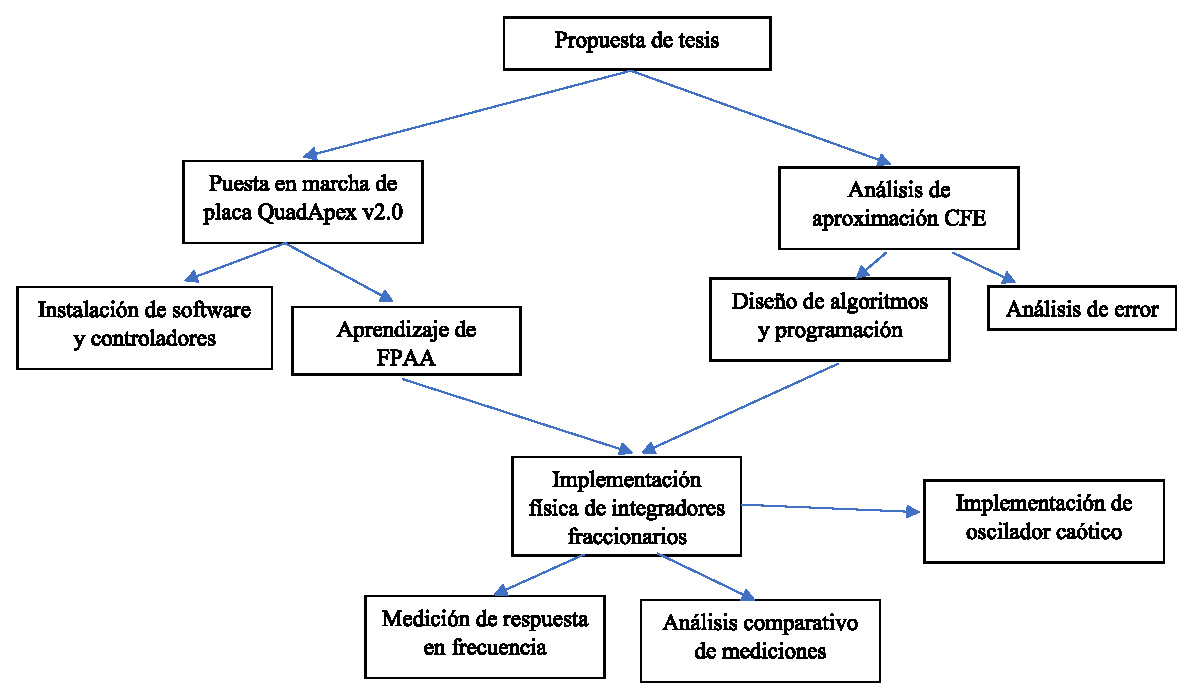
\includegraphics[width = 11cm]{diagrama_de_bloques.eps}
	\caption{Diagrama de bloques}
	\end{figure}
	
	\section{Cronograma de actividades}
	\begin{figure}[hbtp]
	\centering
	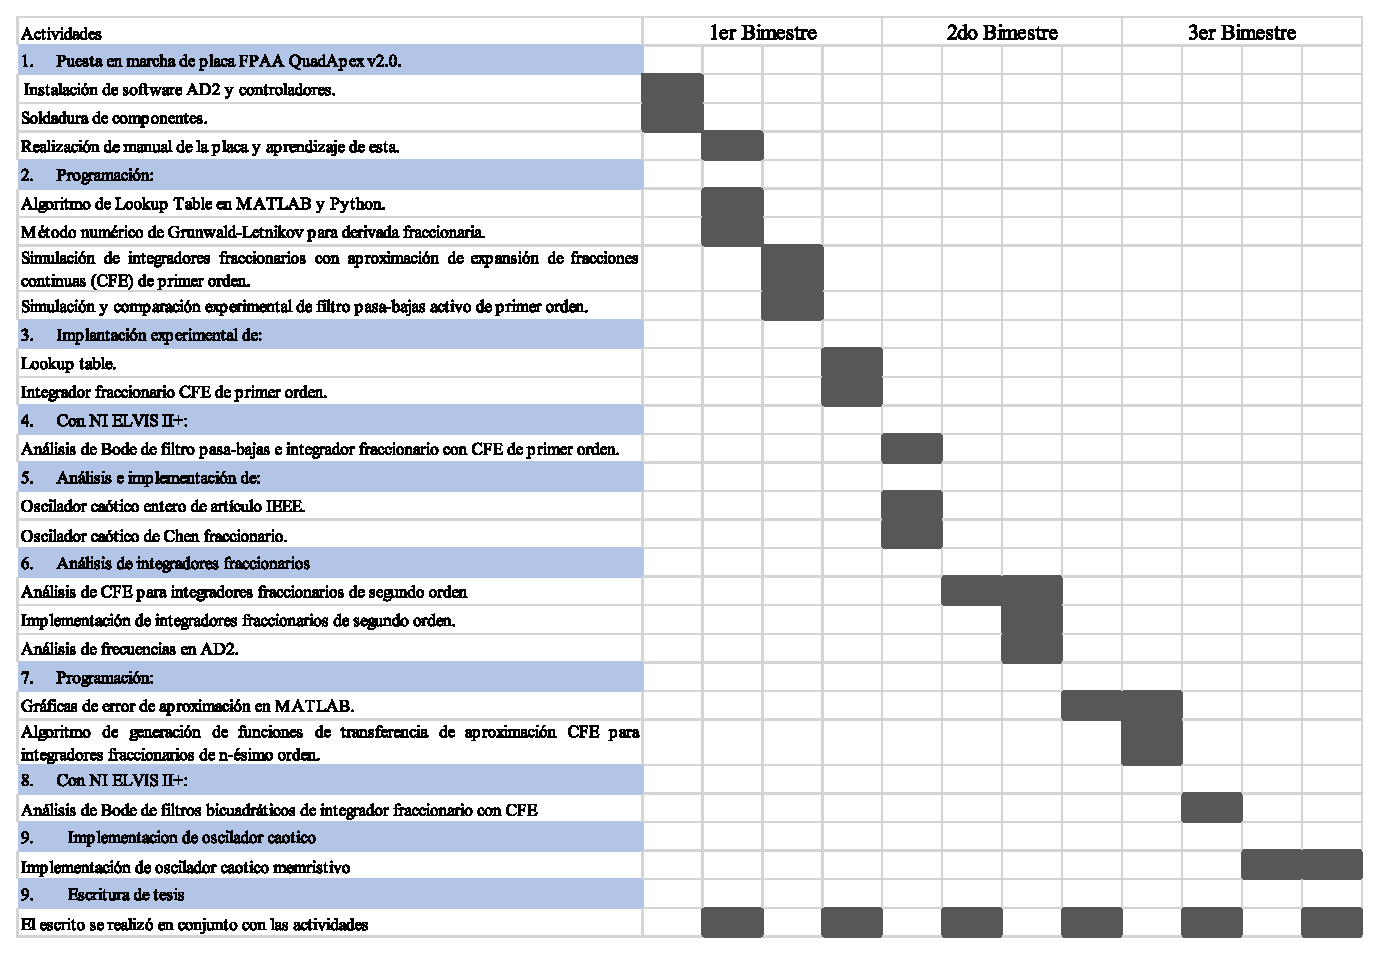
\includegraphics[width = 14.8cm]{cronograma_de_actividades.eps}
	\caption{Cronograma de actividades}
	\end{figure}	
		
%\end{comment}
		
	
	
	
	